\section{Implementation}\label{sec:implementation}


\begin{figure}[t]
\centering
%\begin{pspicture}(8,1.25)
%\showgrid
\rput(1,1.25){\rnode{config}{\parbox{1.3in}{\centering{\mft Router
	Configurations\\ (offline, collected from routers)}}}}
\rput(7,1.25){\rnode{prop}{{\mft Property}}}
\rput(0.25,0.25){\rnode{rs}{\psframebox{\parbox{0.5in}{\centering{\mft Preprocessor}}}}}
\rput(3.3,0.25){\rnode{sim}{\psframebox{\parbox{0.5in}{\centering{\mft Parser}}}}}
\rput(6.65,0.25){\rnode{la}{\psframebox{\parbox{0.5in}{\centering{\mft
	  Verifier}}}}}
\rput(8,0.25){\rnode{end}{}}
\ncline[arrows=->]{rs}{sim}
\ncline[arrows=->]{sim}{la}
\ncline[arrows=->]{la}{end}
\ncarc[arrows=->,nodesep=2pt]{prop}{la}
\ncarc[arrows=->]{config}{rs}
\rput(2.15,0.55){\parbox{0.85in}{{\dft Processed Input}}}
\rput(5,0.55){\parbox{0.55in}{\centering{\dft Intermediate Format}}}
\rput(7.95,0.55){{\dft Error?}}
\end{pspicture}

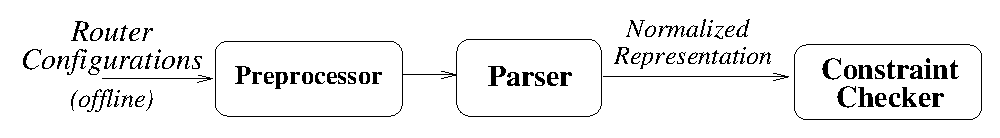
\epsfig{file=rcc/figures/rcc_design.eps, width=\linewidth}
\caption{Overview of \rcc implementation.}
\label{fig:rolex_design}
\end{figure}

\rcc is implemented in 
%about 6,500 lines of 
Perl and has been downloaded
by over seventy network operators.
The parser is roughly
60\% of the code.  
Much of the parser's logic is dedicated to policy
normalization.  
%
Figure~\ref{fig:rolex_design} shows an overview of \rccns, which 
takes as input the set of configuration files collected from
routers in a single AS
using a tool such as ``rancid''~\cite{www-rancid}.
\rcc
converts the vendor-specific BGP configuration to a vendor-independent
normalized 
representation.  It then checks this normalized format for faults
based on a set of correctness constraints.  
\rccns's functionality is
decomposed into three distinct modules: (1)~a preprocessor, which
converts configuration into a more parsable version; (2)~a parser, which
generates the normalized  representation; and (3)~a constraint checker,
which checks the constraints.  



\begin{figure}[t]
\centering
\hspace*{-0.2in}
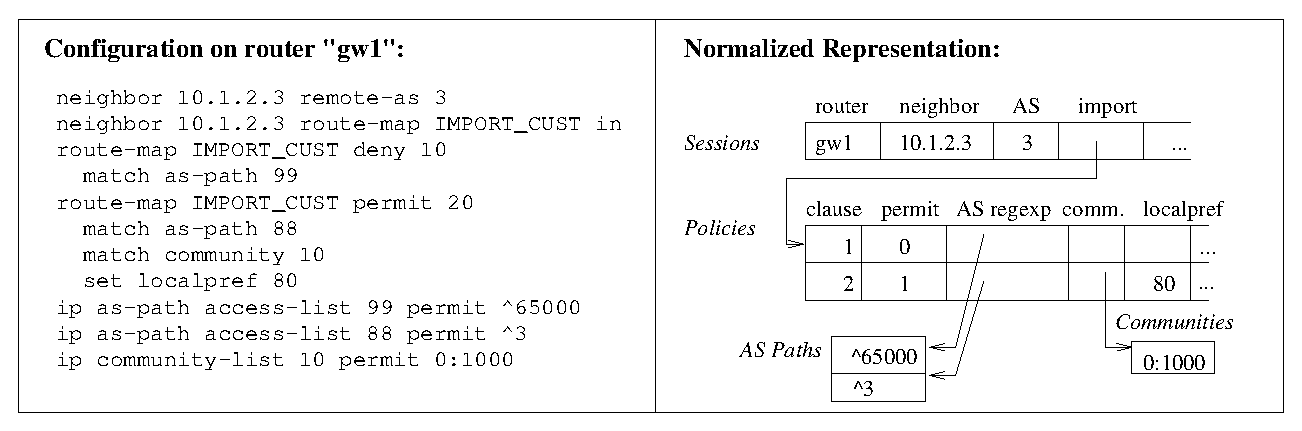
\epsfig{file=rcc/figures/if.eps, width=0.95\linewidth}
\caption{BGP configuration in normalized format.} 
\label{fig:if}
\end{figure}

\subsection{Preprocessing and Parsing}\label{sec:parser}

The {\em preprocessor} adds scoping identifiers to configuration
languages that do not have explicit scoping (\eg, Cisco IOS) and expands
macros (\eg, Cisco's ``peer group'', ``policy list'', and ``template''
options).  After the preprocessor performs some simple checks to
determine whether the configuration is a Cisco-like configuration
or a Juniper configuration, it launches the appropriate parser.  Many
configurations (\eg, Avici, Procket, Zebra, Quarry) resemble Cisco
configuration; the preprocessor translates these configurations so that
they more closely resemble Cisco syntax.

The {\em parser} generates the normalized representation from the
preprocessed configuration.  
%\rcc parses Cisco and
%Juniper configurations, as well as the configurations of other vendors
%that are loosely based on Cisco configuration syntax (\eg, Cisco,
%Procket, Quarry, etc.).  
The parser processes each router's configuration independently.  It
makes a single pass over each router's configuration, looking for keywords
that help determine where in the configuration it is operating (\eg,
``{\tt route-map}'' in a Cisco configuration indicates that the parser
is entering a policy declaration).  The parser builds a table of
normalized policies by
dereferencing all filters and other references in the policy; if the
reference is defined after it is referenced in the same file, the
parser performs lazy evaluation.  When it reaches the end of a file, the
parser flags any policies references in the configuration that it was
unable to resolve.  The parser proceeds file-by-file (taking care to
consider that definitions are scoped by each file), keeping track of
normalized policies and whether they have already appeared in other
configurations. 

Figure~\ref{fig:if} shows \rccns's normalized representation for a
fragment of Cisco IOS.  In \rccns, this normalized representation is
implemented as a set of mySQL database tables corresponding to the
schema shown in Table~\ref{tab:if}.  This Cisco configuration specifies
a BGP session to a neighboring router with IP address {\tt 10.1.2.3} in
AS 3.  This statement is represented by a row in the {\tf sessions}
table.  The second line of configuration specifies that the import
policy (\ie, ``route map'') for this session is defined as ``{\tt
IMPORT\_CUST}'' elsewhere in the file; the normalized representation
represents the import policy specification as a pointer into a separate
table that contains the import policies themselves.  A single policy,
such as {\tt IMPORT\_CUST}, is represented as multiple rows in the {\tf
policies} table.  Each row represents a single clause of the policy.  In
this example, {\tt IMPORT\_CUST} has two clauses: the first rejects all
routes whose AS path matches the regular expression number ``$99$''
(specified as ``{\tt \^{}65000}'' elsewhere in the configuration), and
the second clause accepts all routes that match AS path number ``$88$''
and community number ``$10$'' (\ie, {\tt 0:1000}) and sets the ``local
preference'' 
attribute on the route to a value of $80$.  Each of these clauses is
represented as a row in the {\tf policies} table; specifications for regular
expressions for AS paths and communities are also stored in separate
tables, as shown in Figure~\ref{fig:if}.

\rccns's normalized representation does not store
the names of the policies themselves (\eg, ``{\tt IMPORT\_CUST}'', AS
regular expression number ``88'', etc.).  Rather, the normalized format
only stores a description of what the route policy does (\eg, ``set the
local preference value to $80$ if the AS path matches regular expression
{\tt \^{}3}'').  Two policies may be written using entirely different
names, regular expression numbers, or even in different languages, but
if the policies perform the same operations, \rcc will recognize that
they are in fact the same policy.

%This process of {\em policy canonicalization} makes
%distinguishing policies across multiple routers trivial.  Without this
%normalization, ``eyeballing'' router configurations is not
%easy: policies that have the same name on two different routers may
%perform entirely different operations, and vice versa.  
%We have observed
%this practice surprisingly often.





%% Thus, even if two
%% policies are named differently on two different routers, the
%% canonicalization will reveal that the policies are identical.
%% The parser also recognizes when policies on routers with the
%% same names and reference names are different when the policies actually
%% perform different operations.

%% The {\tf global options}, {\tf sessions}, and {\tf prefixes} tables are
%% populated from statements within the BGP section of the configuration
%% files (\eg, {\tt router bgp} in Cisco configuration).  Other tables are
%% populated by parsing the appropriate sections of the configuration.
%% Populating the {\tf policies} and {\tf filters} tables is more
%% complicated.  \rcc compares policies {\em across} routers; thus, it
%% requires a concise, normalized, step-by-step policy specification.  This
%% process generates a normalized ``pseudocode'' representation of each
%% policy so that policies can be compared across routers.  This process
%% requires dereferencing every variable that is specified in the policy
%% (\ie, community-lists, AS path lists, etc.).  The parser inserts every
%% variable that a policy references that it cannot resolve into the {\tf
%% undefined references} table and joins these normalized policies with the
%% {\tf sessions} table.

\subsection{Constraint Checking}\label{sec:verifier}

\rcc implements constraints that detect each problem in
Table~\ref{tab:rcc_tests} by executing SQL queries against the
normalized format and analyzing the results of these queries in Perl.
%The tests for
%iBGP signaling are about 700 lines of Perl, but most other tests are
%fewer than 30 lines of Perl each.

\rcc checks many constraints by executing simple queries against the
normalized representation.  Checking constraints against the normalized
representation is simpler than analyzing distributed router
configurations.  Consider the test in Table~\ref{tab:rcc_tests} called
``iBGP 
configured on one end''; this constraint requires that, if a router's
configuration specifies an iBGP session to some IP address, then
(1)~that IP address should be the loopback address of some other router
in the AS, and (2)~that other router should be configured with an iBGP
session back to the first router's loopback address.  \rcc tests this
constraint as a single, simple ``select'' statement that ``joins'' the
{\tf loopbacks} and {\tf sessions} tables.  Other tests, such as
checking properties of the iBGP signaling graph, require reconstructing
the iBGP signaling graph using the {\tf sessions} table, a task that is
much easier than examining dependencies across a large set of router
configuration files.

As another example, to check that no
routing policy in the AS prepends any AS number other than its own, \rcc
executes a ``select'' 
query on a join of the {\tf sessions} and {\tf policies} tables that
returns the ASes that each policy prepends (if any) and the routers
where each policy is used. \rcc then checks the {\tf global} table to
ensure that for each router, the AS number configured on the router
matches the ASes that any policy on that router prepends.
